\documentclass[11pt,a4paper]{article}
\usepackage[T1]{fontenc}
\usepackage{lmodern,microtype,graphicx,xcolor}
\usepackage[margin=22mm,top=19mm,bottom=20mm]{geometry}
\usepackage{enumitem,titlesec,caption,fancyhdr,hyperref}
\hypersetup{hidelinks,pdftitle={PACE: Peer-Wise Calibrated Experts for IoT Intrusion Detection with Benign-Only Target Data},pdfauthor={Salaheddine Naslouby, Mohamed Lachgar, Hamid Hrimech}}
\setlength{\parindent}{0pt}
\setlength{\parskip}{3pt}
\setlength{\topsep}{1pt}
\titleformat{\section}{\large\bfseries}{\thesection}{.55em}{}
\titlespacing*{\section}{0pt}{9pt}{5pt}
\captionsetup{font=small,labelfont=bf,labelsep=period,skip=5pt,hypcap=false}
\setlist[enumerate]{leftmargin=1.6em,itemsep=9pt,topsep=5pt,parsep=0pt}
\pagestyle{fancy}
\fancyhf{}
\fancyfoot[C]{\footnotesize\thepage}
\renewcommand{\headrulewidth}{0pt}
\renewcommand{\footrulewidth}{0pt}
\clubpenalty=10000
\widowpenalty=10000
\newcommand{\topic}[1]{\textbf{#1}\enspace}
\begin{document}
\fontsize{10.5}{12.7}\selectfont
\begin{center}
{\fontsize{19}{23}\selectfont\bfseries PACE: Peer-Wise Calibrated Experts for IoT Intrusion Detection with Benign-Only Target Data\par}
\vspace{9pt}
{\normalsize Salaheddine Naslouby$^1$, Mohamed Lachgar$^2$, Hamid Hrimech$^1$\par}
\vspace{4pt}
{\small
$^1$Hassan First University, National School of Applied Sciences (ENSA),\\
LAMSAD Laboratory, Berrechid, Morocco\par
\vspace{2pt}
$^2$Cadi Ayyad University, Higher Normal School (ENS),\\
L2IS Laboratory, Marrakech, Morocco\par}
\end{center}

An IoT monitoring target may have access to normal traffic but no locally labelled attack examples, limiting the use of target-specific supervised intrusion detection. Existing classifiers from other clients can provide attack knowledge, but merging their predictions may suppress useful evidence. At the same time, attacks missed by those classifiers may still appear anomalous relative to the target's legitimate behavior.

PACE (Peer-Wise Calibrated Experts) introduces a target-adaptive intrusion-detection framework that combines these two sources of information without requiring target attack labels. Its calibration algorithm preserves individual peer decisions, while a protected local anchor and heterogeneous expert bank provide complementary anomaly detection.

\section*{PACE: Architecture and Calibration Algorithm}
\begin{center}
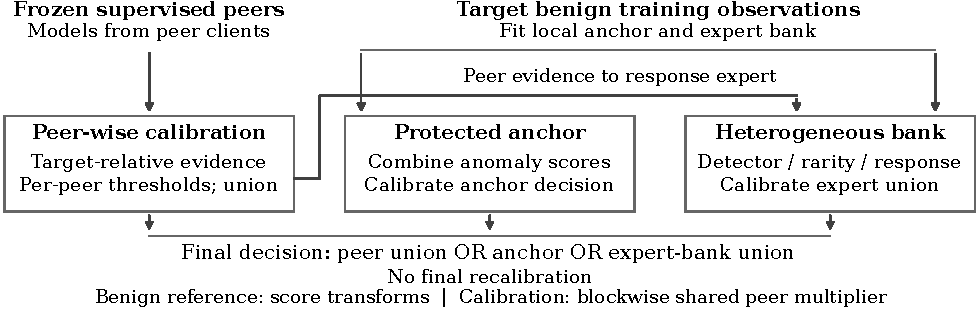
\includegraphics[width=\linewidth]{figures/architecture.pdf}
\captionof{figure}{Frozen peer classifiers supply attack evidence; benign target observations support local fitting, reference transformations, and calibration. Peer-wise thresholds, a protected anchor, and an expert bank retain three alert routes through the final decision.}
\end{center}

\topic{Peer-wise calibration.} Conventional score fusion can let one peer's score distribution dominate the final threshold and obscure another's evidence [3]. PACE instead transforms and calibrates each peer's evidence against benign target observations. Blockwise calibration adjusts a shared multiplier on the peer union while retaining the individual alert decisions.

\topic{Complementary local detection.} The protected anchor retains a separately calibrated decision from aggregated anomaly scores. The heterogeneous bank adds detector-specific responses, feature rarity, and anomalies in peer-response patterns. Both use benign target observations and can detect attacks outside the peer union.

\topic{Integrated decision algorithm.} The calibrated peer union ($U_P$), protected anchor ($U_A$), and expert-bank union ($U_B$) retain separate decisions. Any route can trigger an alert, combining supervised attack knowledge and local anomalies without collapsing them into one score.
\[
D(x)=U_P(x)\lor U_A(x)\lor U_B(x).
\]
PACE integrates individually calibrated foreign classifiers with complementary local anomaly decisions under a common target-adaptation procedure. Unlike score fusion [3] and calibrated hybrids such as MCDE and Nweke [1,2], the peer, anchor, and bank routes remain separate through inference. Together, peer-wise calibration and complementary local decisions define a unified inference procedure that combines transferred attack knowledge with target-specific anomaly evidence.

\newpage
\section*{Experimental Validation}
PACE was evaluated on 58 targets from six IoT security datasets, using three learning seeds and two primary local fitting budgets. The evaluation examines overall detection performance, the effect of peer-wise calibration, and the contribution of complementary local anomaly evidence.

PACE improves detection over the shared-peer mean-local comparator in all four primary configurations, with gains ranging from 2.32 to 2.83 percentage points. All four paired confidence intervals exclude zero. At $\alpha=0.05$, the improvements also accompany lower mean false-positive rate (FPR) at both local fitting budgets. With 400 fitting rows, detection increases from 87.36\% to 89.68\%, while mean FPR decreases from 6.44\% to 5.43\%.

\begin{center}
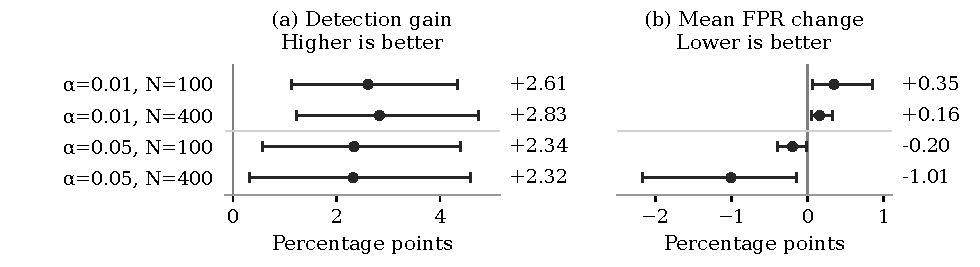
\includegraphics[width=\linewidth]{figures/primary-comparison.pdf}
\captionof{figure}{PACE minus the shared-peer mean-local comparator in all four primary settings. $N$: local fitting rows; pp: percentage points. Higher detection gains and lower false-positive-rate (FPR) changes are better. Whiskers show paired 95\% corpus-stratified bootstrap intervals over seed-averaged targets.}
\end{center}

With PACE's complete local branch fixed, peer-wise calibration gains 4.47 percentage points over mean fusion and 3.16 over maximum fusion. Higher mean FPR accompanies these additional detections, quantifying the operating trade-off from retaining separate peer evidence.

\begin{center}
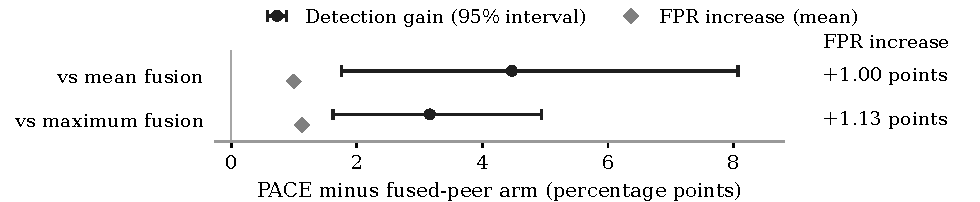
\includegraphics[width=\linewidth]{figures/peer-fusion.pdf}
\captionof{figure}{Peer-wise calibration with the local branch fixed ($\alpha=0.05$, $N=400$). Circles: detection gains with paired 95\% intervals; diamonds: mean FPR increases (point estimates).}
\end{center}

Local routes recover attacks missed by the peer union: at $\alpha=0.01$, $N=400$, local-exclusive detection averages 14.74\% in TON\_IoT and 12.10\% in IoT-23. These detections illustrate the complementary role of benign-only local models, which provide attack coverage beyond that of the transferred supervised classifiers. These are coverage fractions, not comparator gains. Rarity-family removal produces the largest loss among tested expert-family removals. Coverage and detection average attack types, seeds, and targets; FPR averages seeds and targets.

\section*{Conclusion}
PACE's complete local architecture improves detection across all four primary settings, with lower mean FPR at both $\alpha=0.05$ budgets. Separate peer-fusion experiments quantify the additional detection and false-alert cost of retaining individual peer decisions. Together, these findings support combining transferred attack knowledge with complementary benign-only target evidence.

The results concern the evaluated benchmark, and empirical calibration does not guarantee future false-positive rates.

\vfill
{\footnotesize\setlength{\parskip}{2pt}\textbf{References}\par
[1] Yue et al. Calibrated dual evidence for unseen IoT attacks (MCDE). \textit{Entropy} 28, 1026 (2026).\par
[2] Nweke. Tail-calibrated mixture of experts for IEC 61850 intrusion detection. \textit{Discover Computing} 29, 434 (2026).\par
[3] Zimek et al. Ensembles for unsupervised outlier detection. \textit{ACM SIGKDD Explorations} 15(1), 11--22 (2014).}
\end{document}
